\documentclass[12pt, titlepage]{article}

\usepackage{graphicx} % Allows for images
\usepackage{wrapfig} % Allows for text wrapping around images
\usepackage{hyperref} % Allows for hyperlinks
\usepackage{siunitx} % Allows for SI units
\usepackage{amsmath} % Allows for math
\usepackage{enumerate} % Allows for custom enumerations
\usepackage{xcolor} % Allows for custom colors
\usepackage{tikz, tcolorbox} % Allows for custom boxes
\usepackage{microtype} % Allows for better text alignment
\usepackage{listings} % Allows for code listings
\usepackage{booktabs} % Allows for better tables
\usepackage{float} % Allows for better figure placement
\usepackage{geometry} % Allows for custom page geometry
\usepackage{fancyhdr} % Allows for custom headers and footers
\usepackage{caption} % Allows for custom captions
\usepackage{array} % Required package for specifying column width and line in the table
\usepackage{changepage} % Required for the adjustwidth environment to temporarily widen margins

\fancypagestyle{myarticlestyle}{
    \fancyhf{} % Clear header and footer
    \fancyhead[L]{\leftmark} % Section name on the left
    \fancyhead[R]{\thepage} % Page number on the right
}
\fancypagestyle{tocstyle}{
    \fancyhf{} % Clear header and footer
    \fancyhead[L]{CONTENTS} % Section name on the left
    \fancyhead[R]{\thepage} % Page number on the right
}

\pagestyle{myarticlestyle}
\setlength{\headheight}{15pt}

\begin{document}
\tableofcontents
\listoffigures
\listoftables
\thispagestyle{tocstyle}
\newpage
\section{Objectives}
The behavior of beams under different loading conditions is a fundamental
aspect of structural engineering. Understanding how beams deflect when
subjected to varying loads is crucial in designing safe and efficient
structures. In this experiment, the focus is on two specific beam
configurations: the cantilever and the simply supported beam. The deflection of
these beams will be investigated both theoretically and experimentally.\\[10pt]
The objectives for this experiment are outlined as follows:
\begin{enumerate}
    \item \textbf{Measurement of Deflection:} Experimentally acquire accurate
      values of deflection for both a cantilever and a simply supported beam
      under varying loads to understand their structural behaviors.
    
    \item \textbf{Comparison of Experimental and Theoretical Results:} Analyze
      and compare the obtained experimental deflection values with the
      theoretically predicted values for both the cantilever and the simply
      supported beam to assess the accuracy and reliability of theoretical
      models in predicting structural deflections.
\end{enumerate}

These objectives aim to provide a comprehensive understanding of how different
types of beam structures behave under applied loads and to evaluate the
alignment between theoretical predictions and actual experimental observations
in real-world scenarios.
\newpage
\section{Procedure}
This experiment consists of two parts: the cantilever beam testing and the
simply supported beam testing.
\subsection{Cantilever Beam Testing}
\begin{enumerate}
    \item \textbf{Step 1:} Check the initial readings of the electrical
      potentiometers to ensure they are zero.
    
    \item \textbf{Step 2:} Apply loads in increments of 2 lb (8.9 N) at the
      mid-span (\(P1\)) up to a total load of 10 lb. Record the vertical
      deflections at both the mid-span (\(P1\)) and at the end of the
      cantilever beam (\(P2\)) for each load.
    
    \item \textbf{Step 3:} Remove the applied load.
    
    \item \textbf{Step 4:} Apply the same set of loads to the end of the beam
      (\(P2\)) and measure the deflections at the mid-span (\(P1\)) and at the
      end of the cantilever beam (\(P2\)).
\end{enumerate}

\subsection{Simply Supported Beam Testing}
\begin{enumerate}
    \item \textbf{Step 1:} Ensure that the initial readings of the electrical
      potentiometers are zero.
    
    \item \textbf{Step 2:} Apply loads in increments of 10 lb (44.482 N) at the
      mid-span of the beam (\(P3\)) up to a total load of 40 lb (177.928 N).
      Record the vertical deflections at both the mid-span (\(P3\)) and at the
      quarter-span of the beam (\(P4\)) for each load.
    
    \item \textbf{Step 3:} Remove the applied load.
    
    \item \textbf{Step 4:} Apply the same set of loads to the quarter-span
      (\(P4\)) and measure the deflections at the mid-span (\(P3\)) and at the
      quarter-span of the beam (\(P4\)).
\end{enumerate}
Throughout the experiment, ensure accurate recording of all measurements,
maintain the safety protocols, and perform the tests as per the specified
loading conditions for each beam configuration.
\newpage
\subsection{Free-Body Diagrams}
This section contains the free-body diagrams for the each beam and each loading
condition.
\subsubsection{Cantilever Beam Load Applied at the Mid-Span}
\begin{figure}[H]
    \centering
    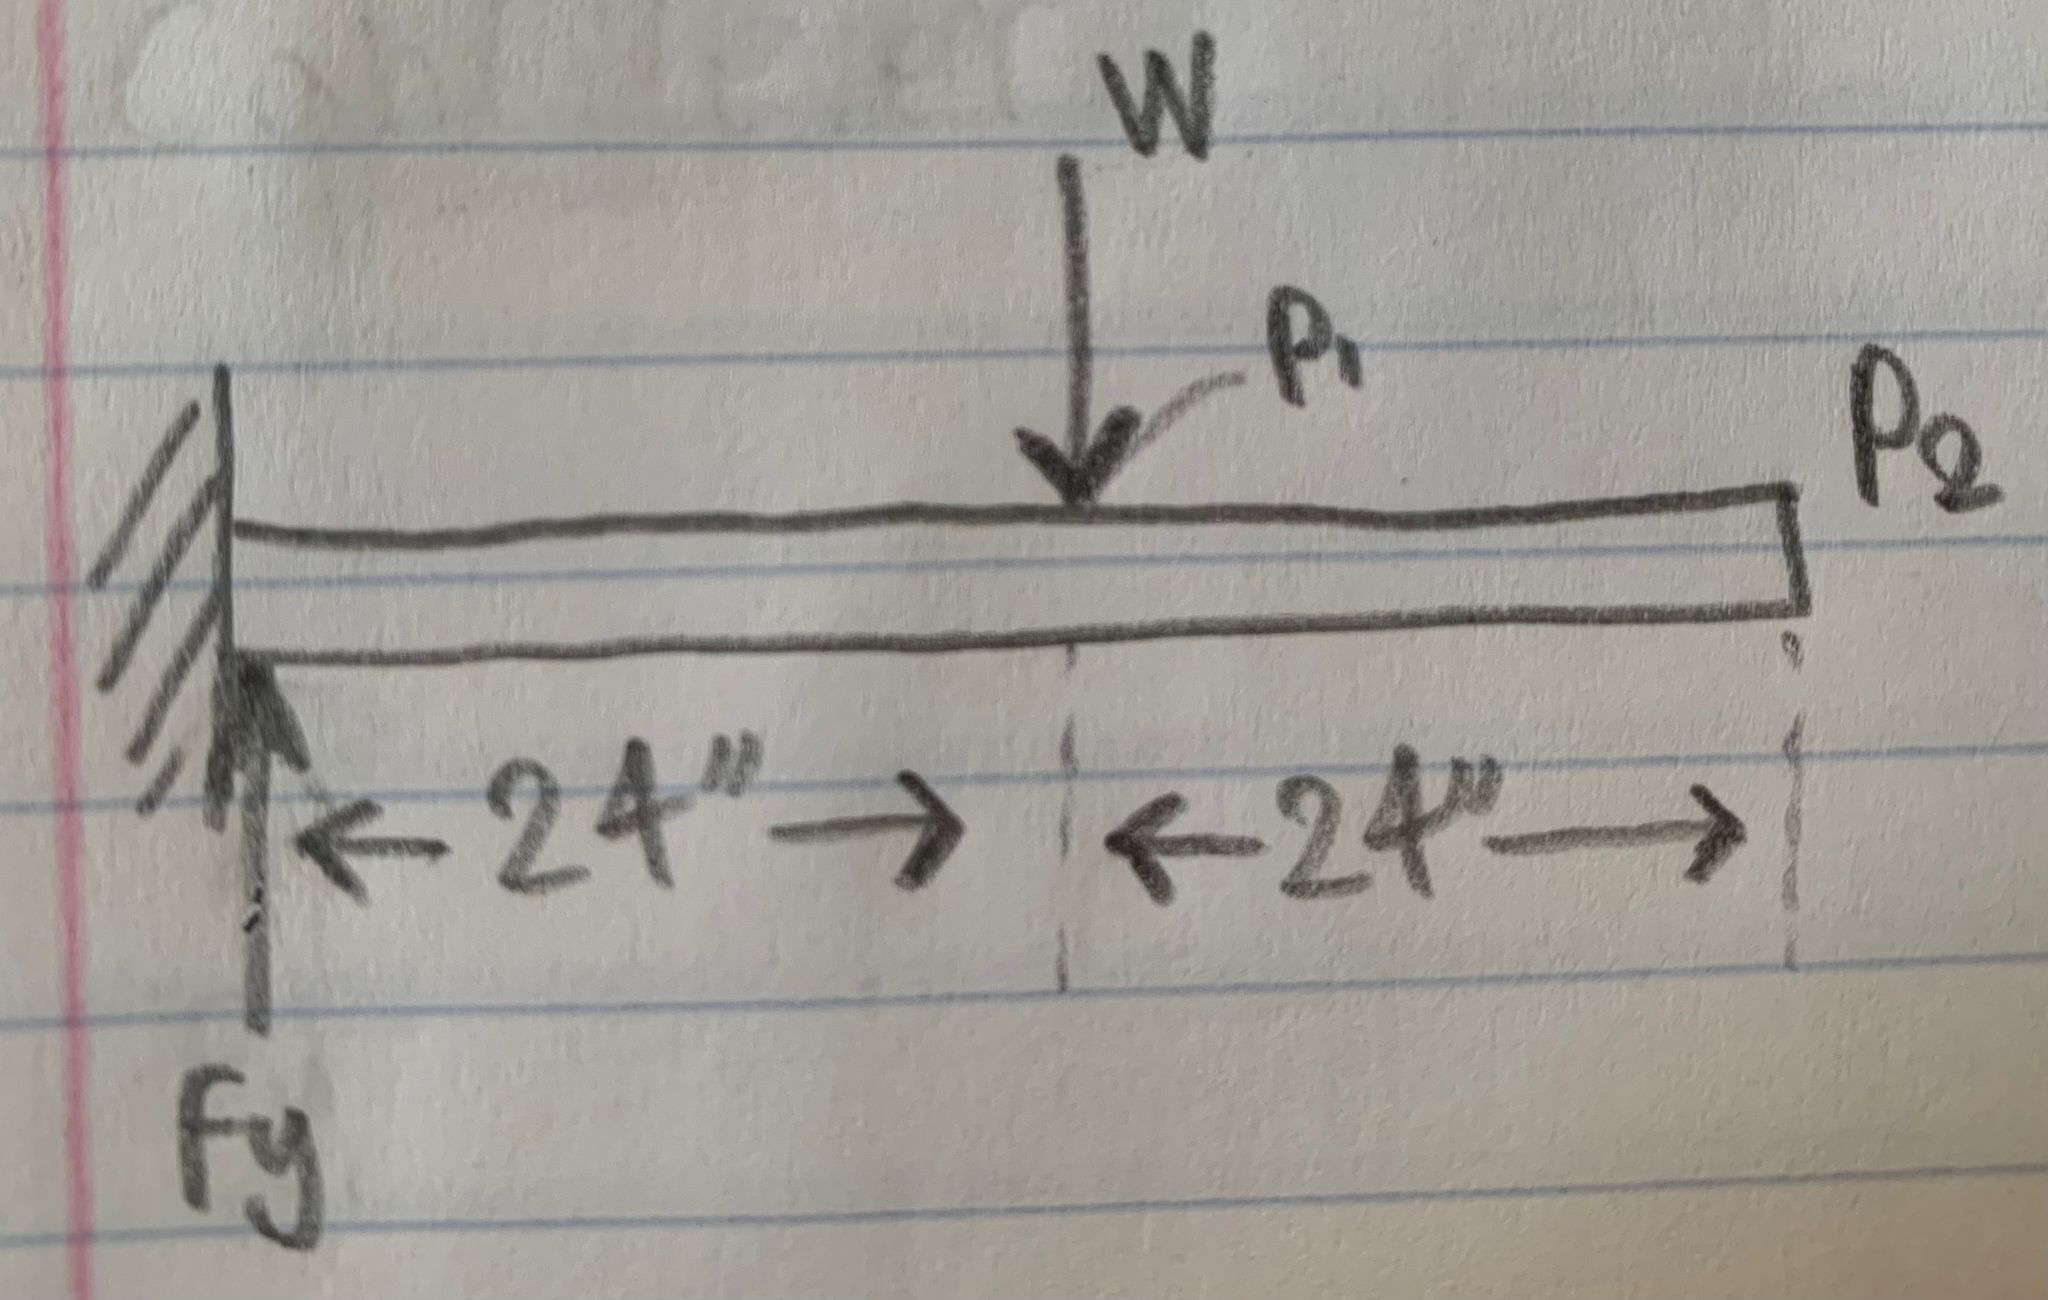
\includegraphics[width=0.6\textwidth]{./Images/C_mid.jpg}
    \caption{Free-body diagram of the cantilever beam with the load applied at
    the mid-span.}
    \label{fig:CantileverBeamMid}
\end{figure}
\subsubsection{Cantilever Beam Load Applied at the End}
\begin{figure}[H]
    \centering
    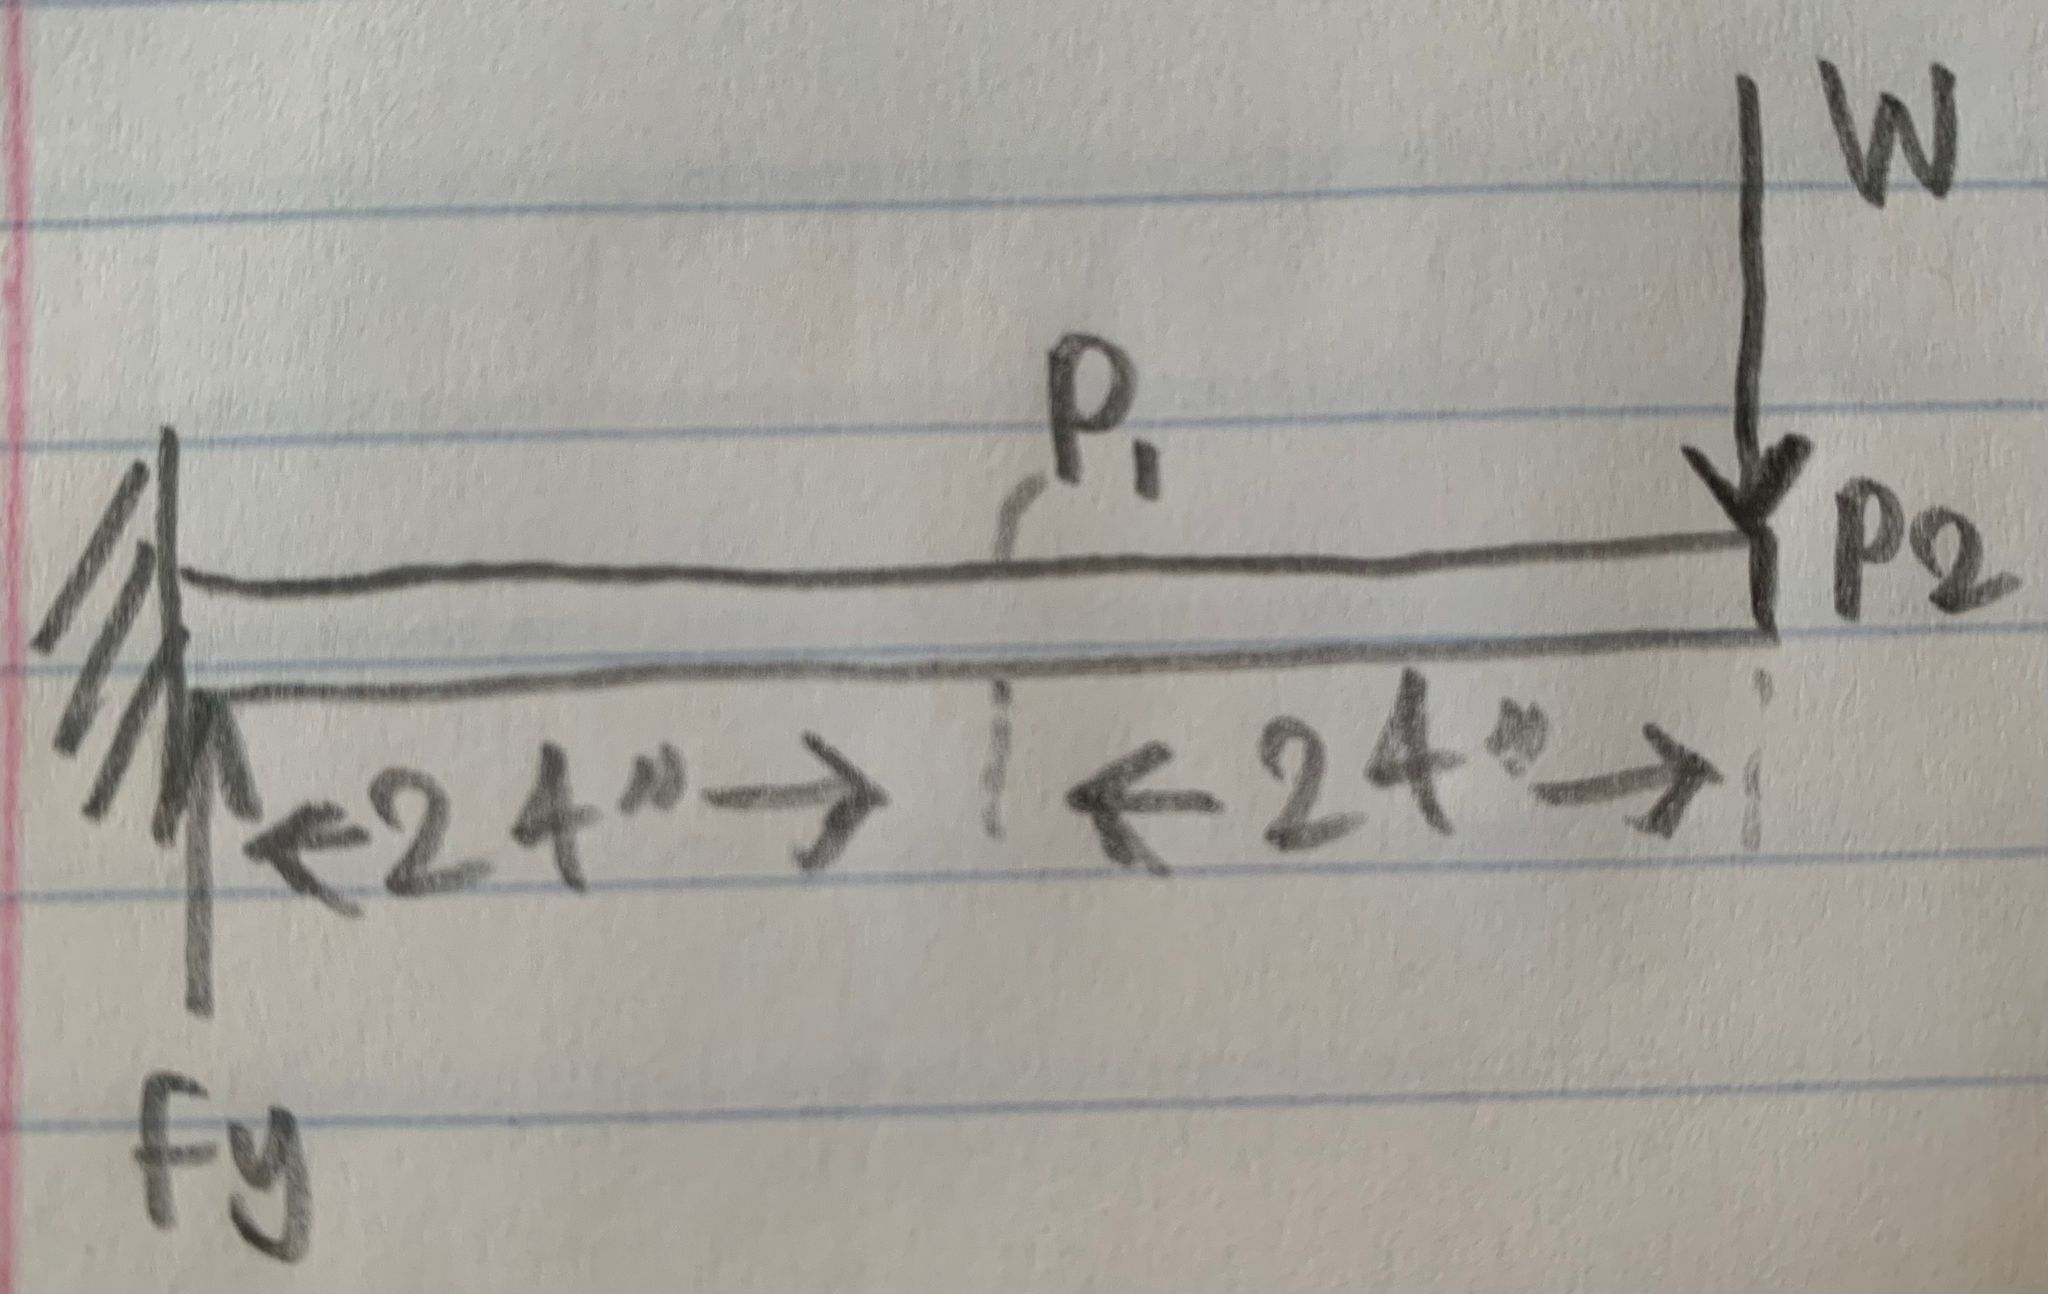
\includegraphics[width=0.6\textwidth]{./Images/C_end.jpg}
    \caption{Free-body diagram of the cantilever beam with the load applied at
    the end.}
    \label{fig:CantileverBeamEnd}
\end{figure}
\subsubsection{Simply Supported Beam Load Applied at the Mid-Span}
\begin{figure}[H]
    \centering
    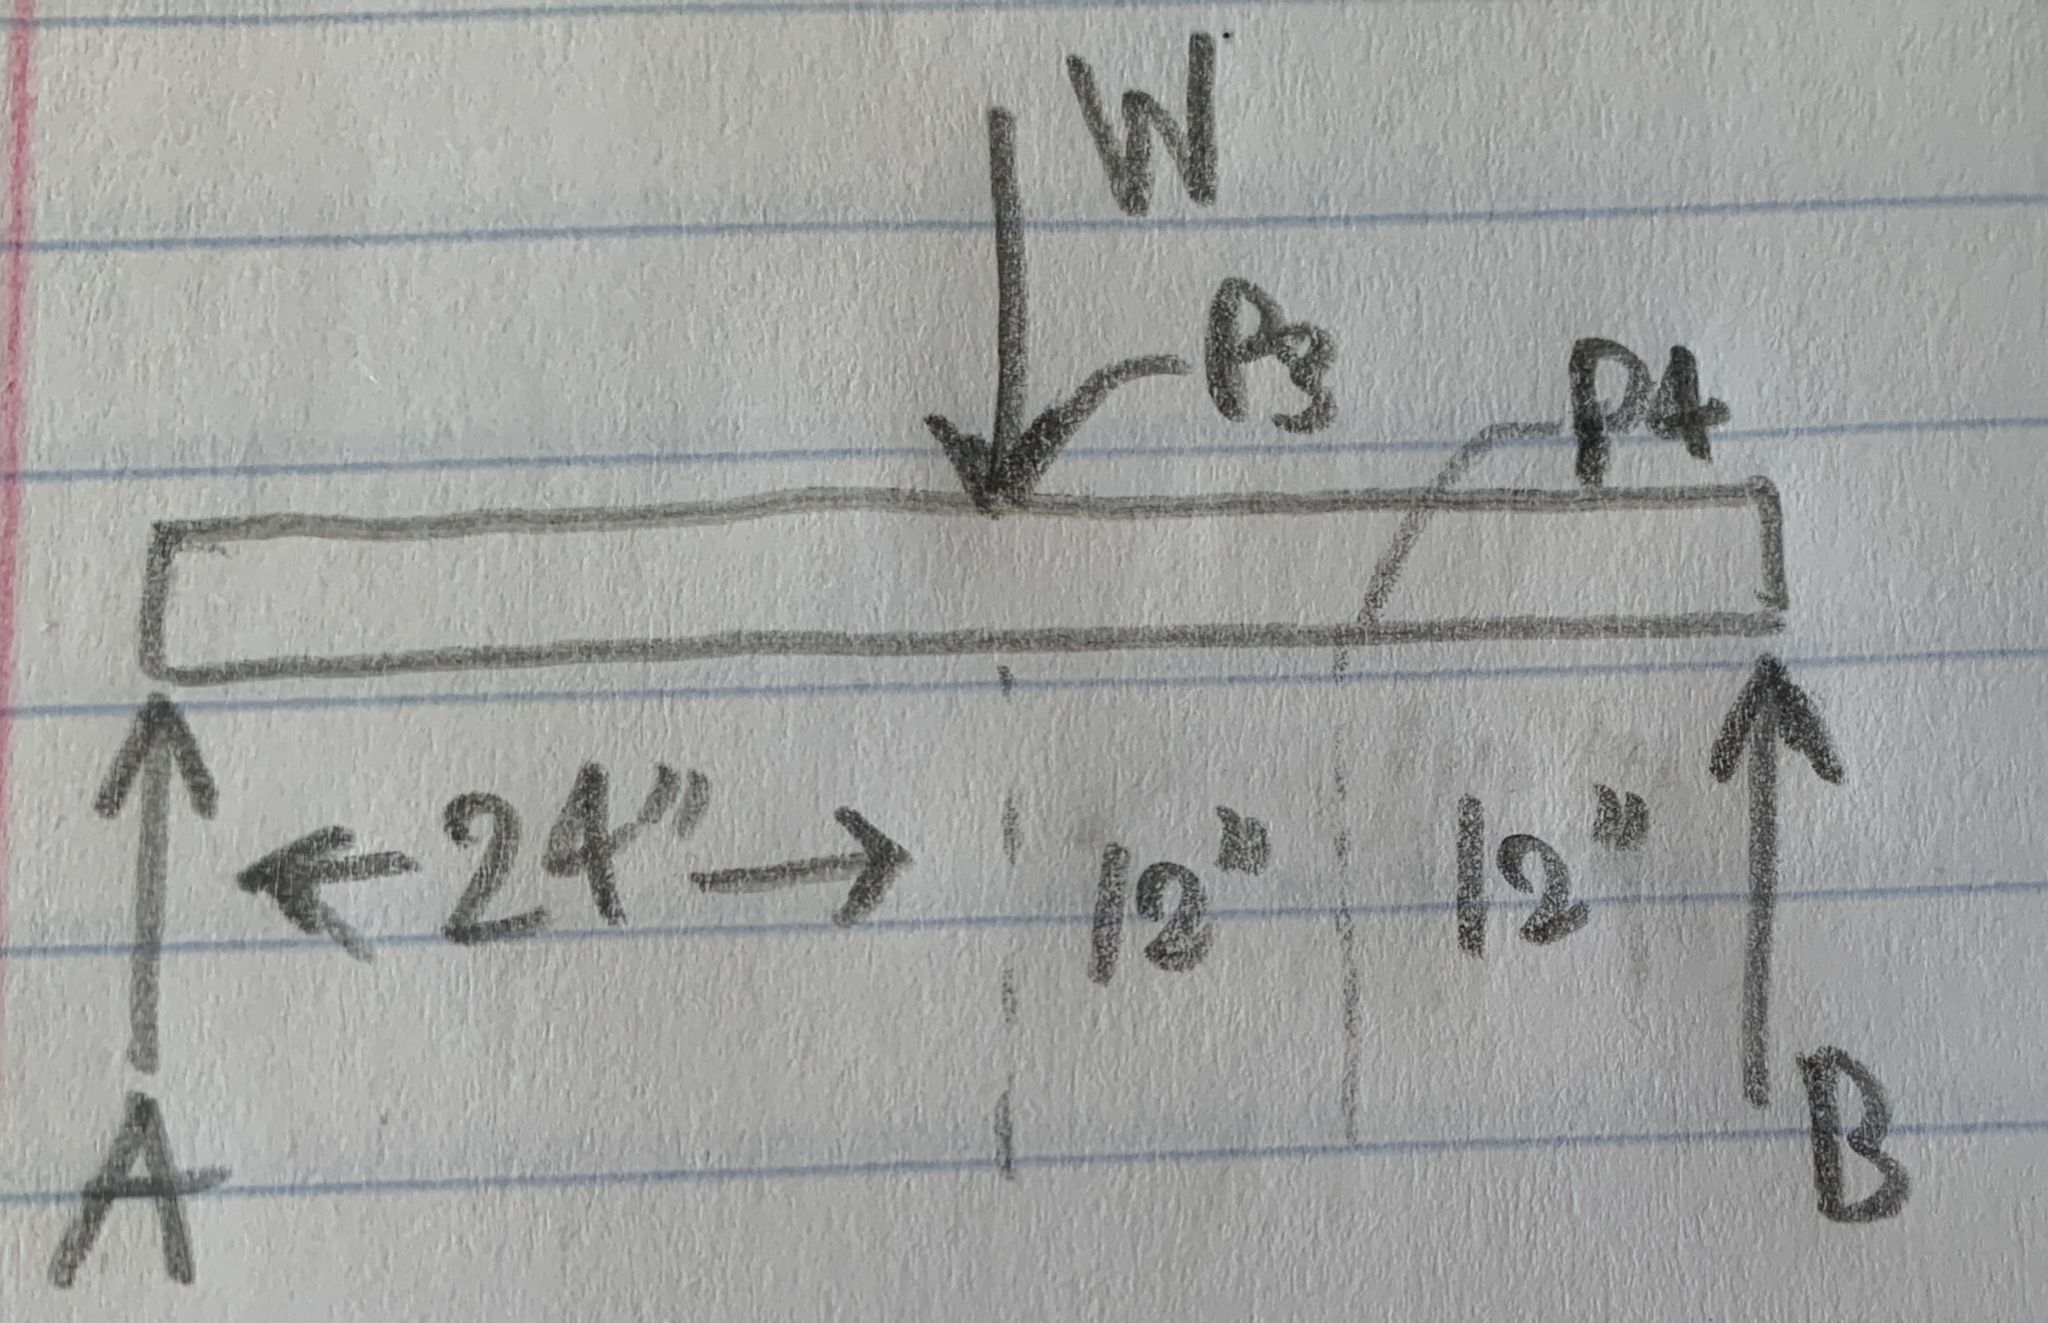
\includegraphics[width=0.6\textwidth]{./Images/S_mid.jpg}
    \caption{Free-body diagram of the simply supported beam with the load
    applied at the mid-span.}
    \label{fig:SimplySupportedBeamMid}
\end{figure}
\subsubsection{Simply Supported Beam Load Applied at the Quarter-Span}
\begin{figure}[H]
    \centering
    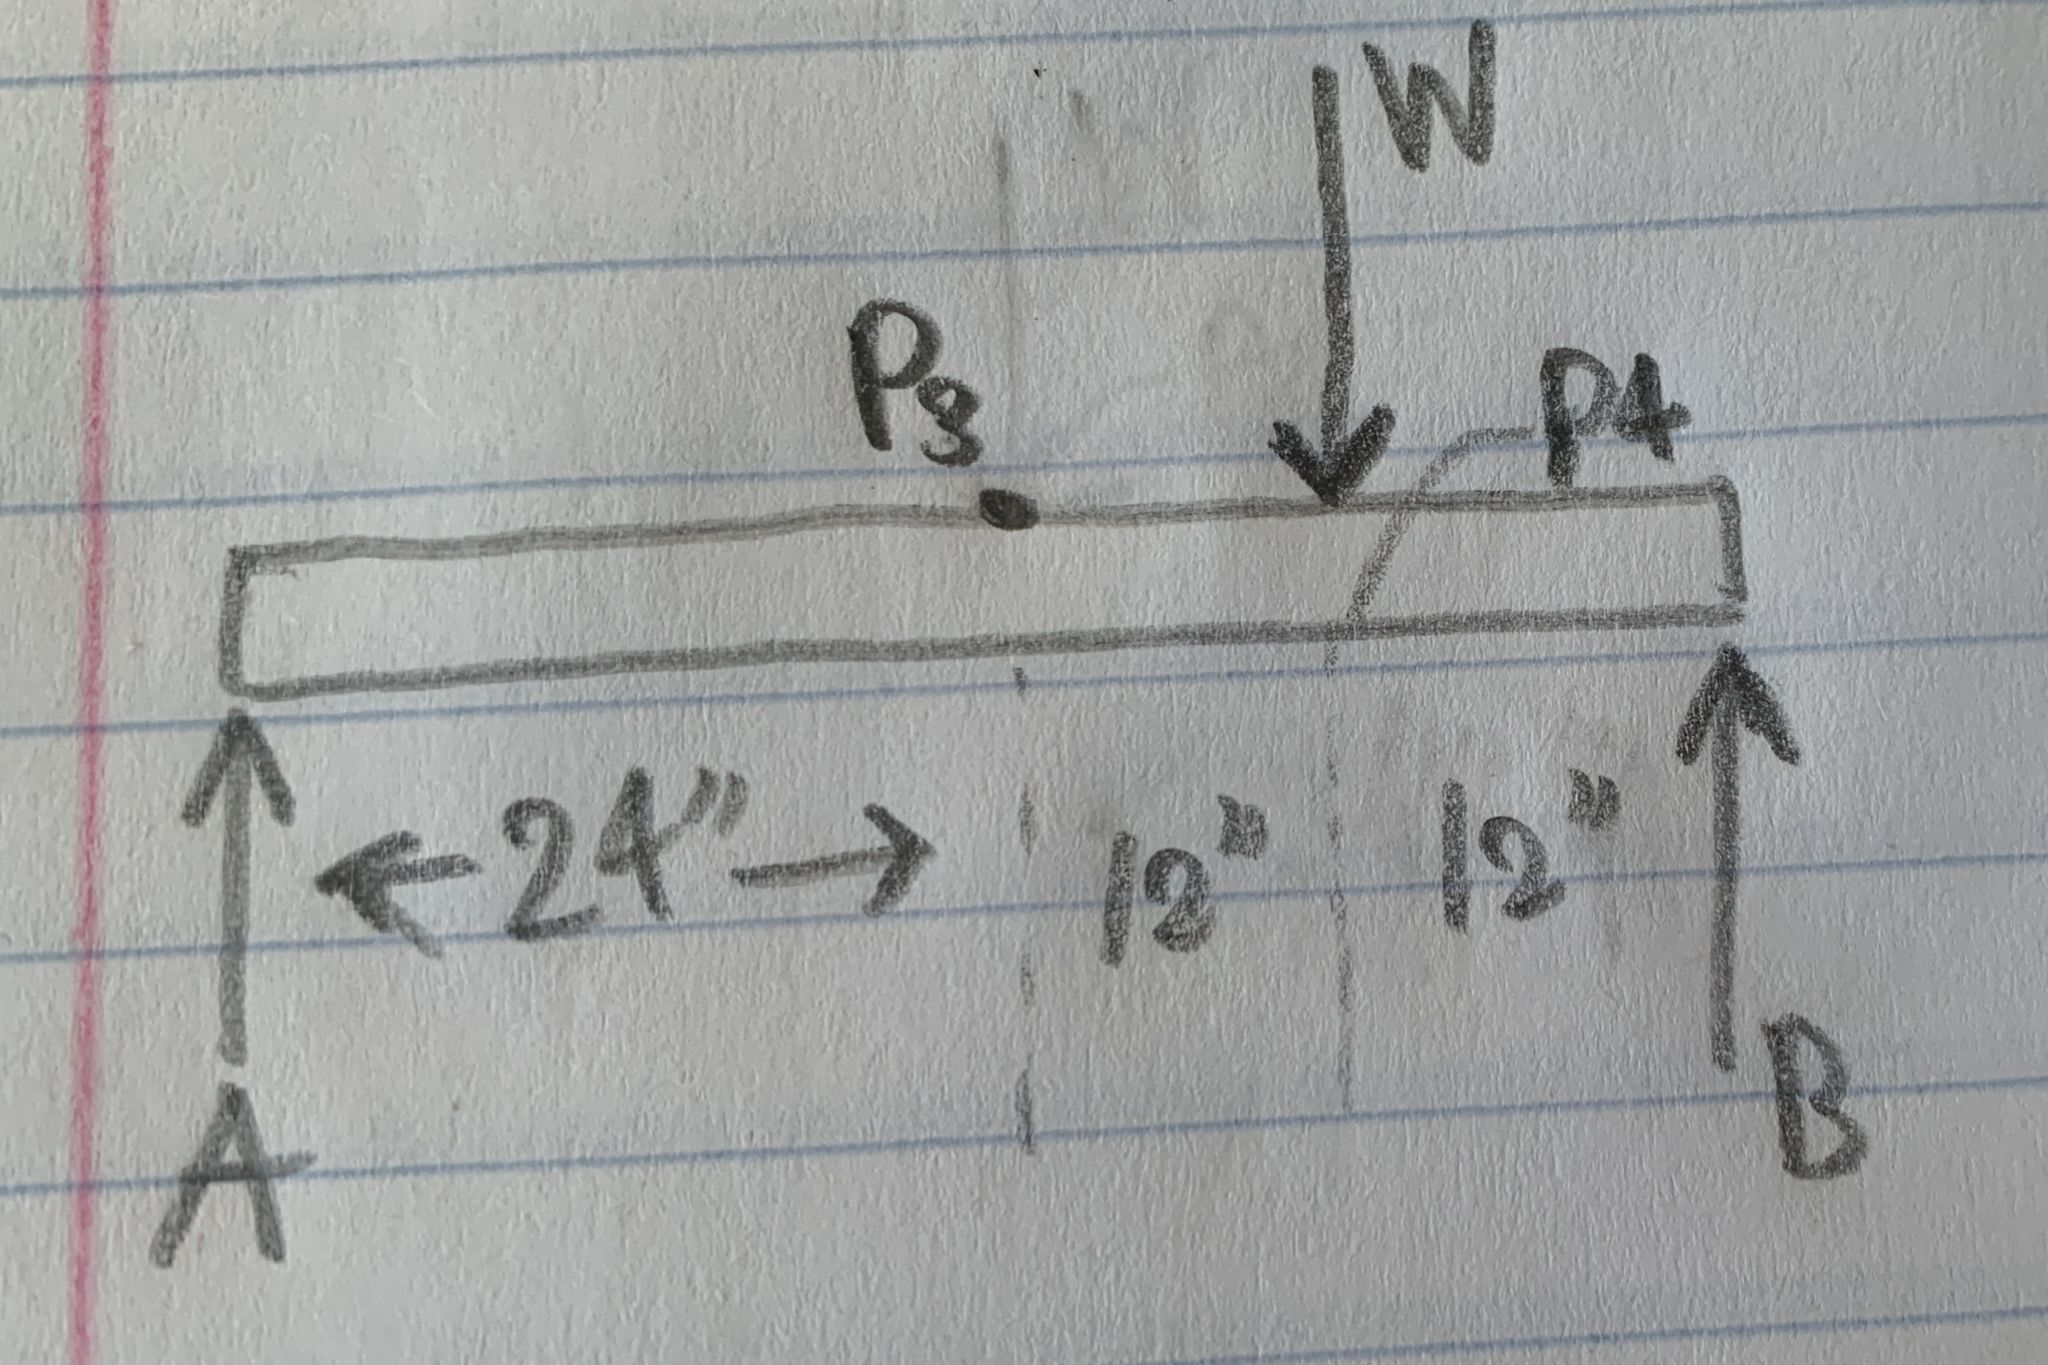
\includegraphics[width=0.6\textwidth]{./Images/S_quarter.jpg}
    \caption{Free-body diagram of the simply supported beam with the load
    applied at the quarter-span.}
    \label{fig:SimplySupportedBeamQuarter}
\end{figure}
\newpage
\section{Results}
This section contains theoretical derivation of the deflection equations for
each beam and each loading condition, the experimental results, and the
plots and summary tables of the theoretical and experimental results in the
comparison section.
\subsection{Cantilever Beam Load Applied at the Mid-Span}
\subsubsection{Theoretical Results}
The calculations for the theoretical deflection of the cantilever beam with the
load applied at the mid-span are shown in figure \ref{fig:TheoreticalCantileverBeamMid}.
\begin{figure}[H]
    \centering
    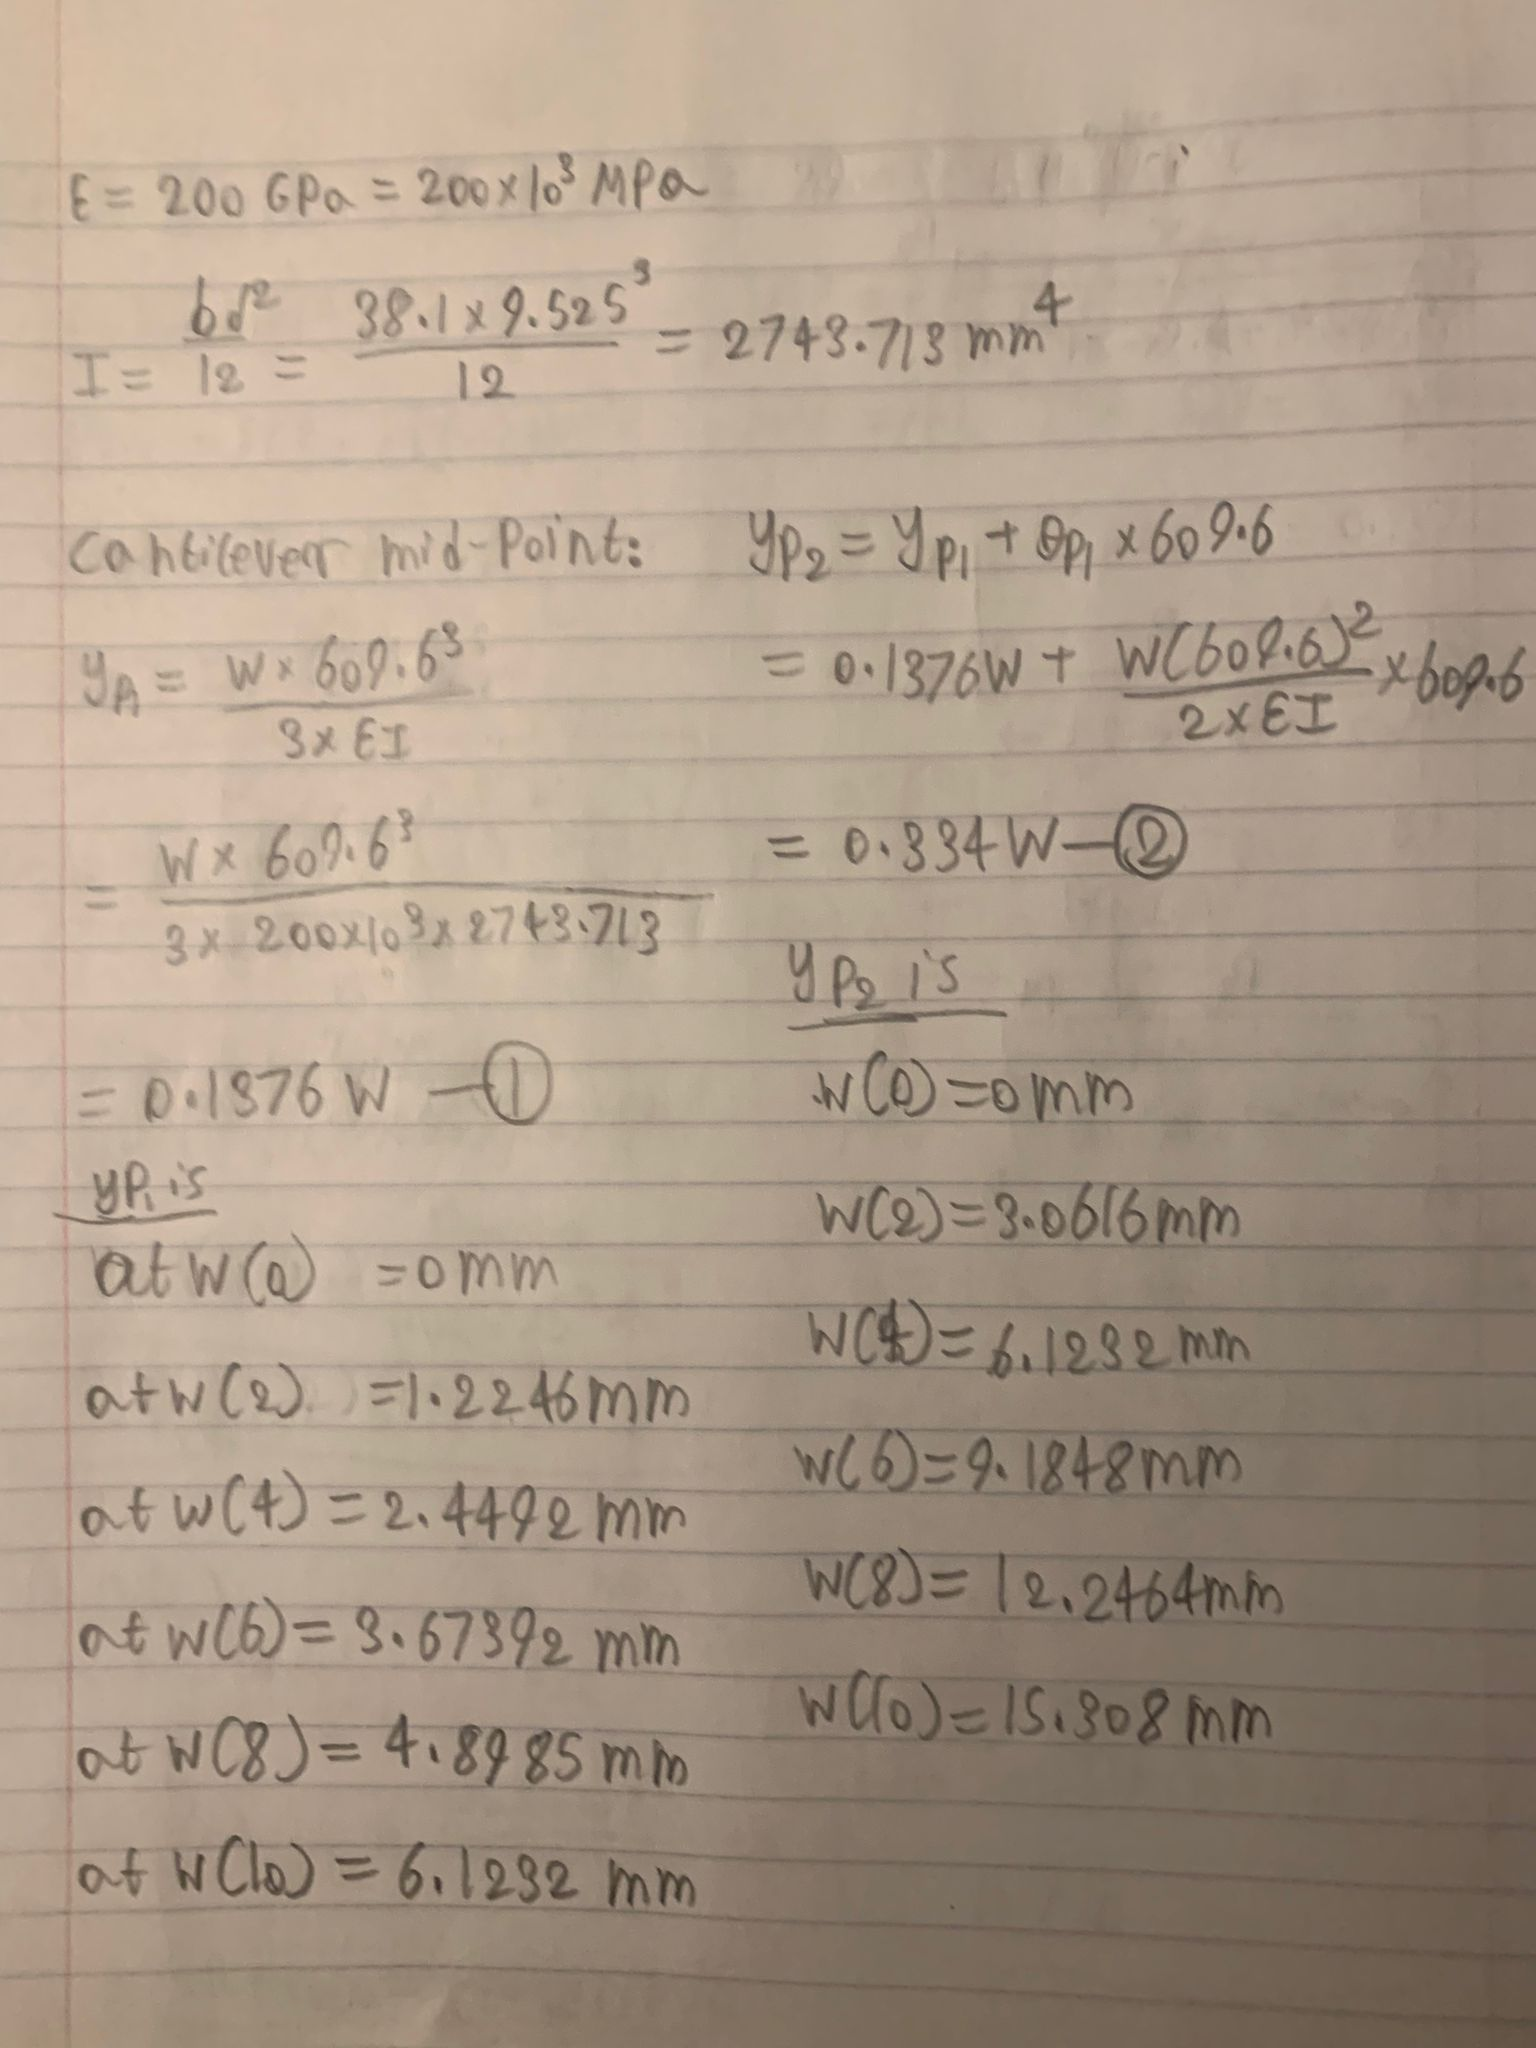
\includegraphics[width=0.6\textwidth]{./Images/C_M.jpeg}
    \caption{Theoretical deflection of the cantilever beam at the mid-span}
    \label{fig:TheoreticalCantileverBeamMid}
\end{figure}
\subsubsection{Experimental Results}
The experimental results for the deflection of the cantilever beam with the
load applied at the mid-span are shown in table \ref{tab:ExperimentalCantileverBeamMid}.
\begin{table}[H]
    \centering
    \caption{Experimental deflection of the cantilever beam at the mid-span}
    \label{tab:ExperimentalCantileverBeamMid}
    \begin{tabular}{|c|c|c|}
        \hline
        \textbf{Load (lb)} & \textbf{Deflection P1 (in)} & \textbf{Deflection P2 (in)}\\
        \hline
        2 & -0.096259843 & -0.305385827 \\
        \hline
        4 & -0.19707874 & -0.616444882 \\
        \hline
        6 & -0.29834252 & -0.917594488 \\
        \hline
        8 & -0.413007874 & -1.239968504 \\
        \hline
        10 & -0.513062992 & -1.530185039 \\
        \hline
    \end{tabular}
\end{table}
\subsubsection{Comparison of Theoretical and Experimental Results}
To compare the theoretical and experimental results, the theoretical deflection
values and the experimental deflection values are shown in table \ref{tab:ComparisonCantileverBeamMid}.
\begin{table}[H]
  \centering
  \caption{Comparison of theoretical and experimental deflection of the cantilever beam at the mid-span}
  \label{tab:ComparisonCantileverBeamMid}
  \begin{adjustwidth}{-1in}{-1in}
    \begin{tabular}{|c|c|c|c|}
        \hline
        \textbf{Load (lb)} & \textbf{Theoretical Deflection (in)} & \textbf{Experimental Deflection (in)} & \textbf{Percentage Error (\%)} \\
        \hline
        0 & 0 & 0 & 0 \\
        \hline
        2 & -0.120525977 & -0.096259843 & 20.13 \\
        \hline
        4 & -0.241051954 & -0.19707874 & 18.24 \\
        \hline
        6 & -0.361577931 & -0.29834252 & 17.49 \\
        \hline
        8 & -0.482103908 & -0.413007874 & 14.33 \\
        \hline
        10 & -0.602629885 & -0.513062992 & 14.86 \\
        \hline
    \end{tabular}
  \end{adjustwidth}
\end{table}
\newpage
The difference is also plotted in figure \ref{fig:ComparisonCantileverBeamMid}.
\begin{figure}[H]
    \centering
    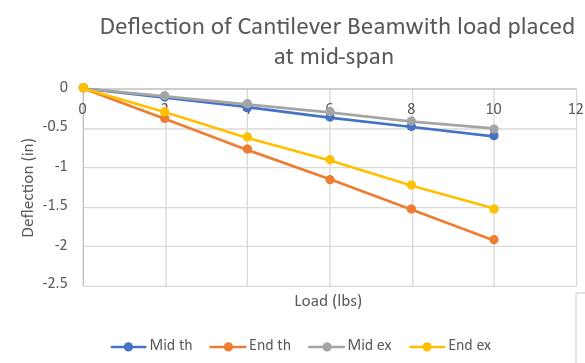
\includegraphics[width=0.9\textwidth]{./Images/C_M_C.png}
    \caption{Comparison of theoretical and experimental deflection of the cantilever beam at the mid-span}
    \label{fig:ComparisonCantileverBeamMid}
\end{figure}
\newpage
\subsection{Cantilever Beam Load Applied at the End}
\subsubsection{Theoretical Results}
The calculations for the theoretical deflection of the cantilever beam with the
load applied at the end are shown in figure \ref{fig:TheoreticalCantileverBeamEnd}.
\begin{figure}[H]
    \centering
    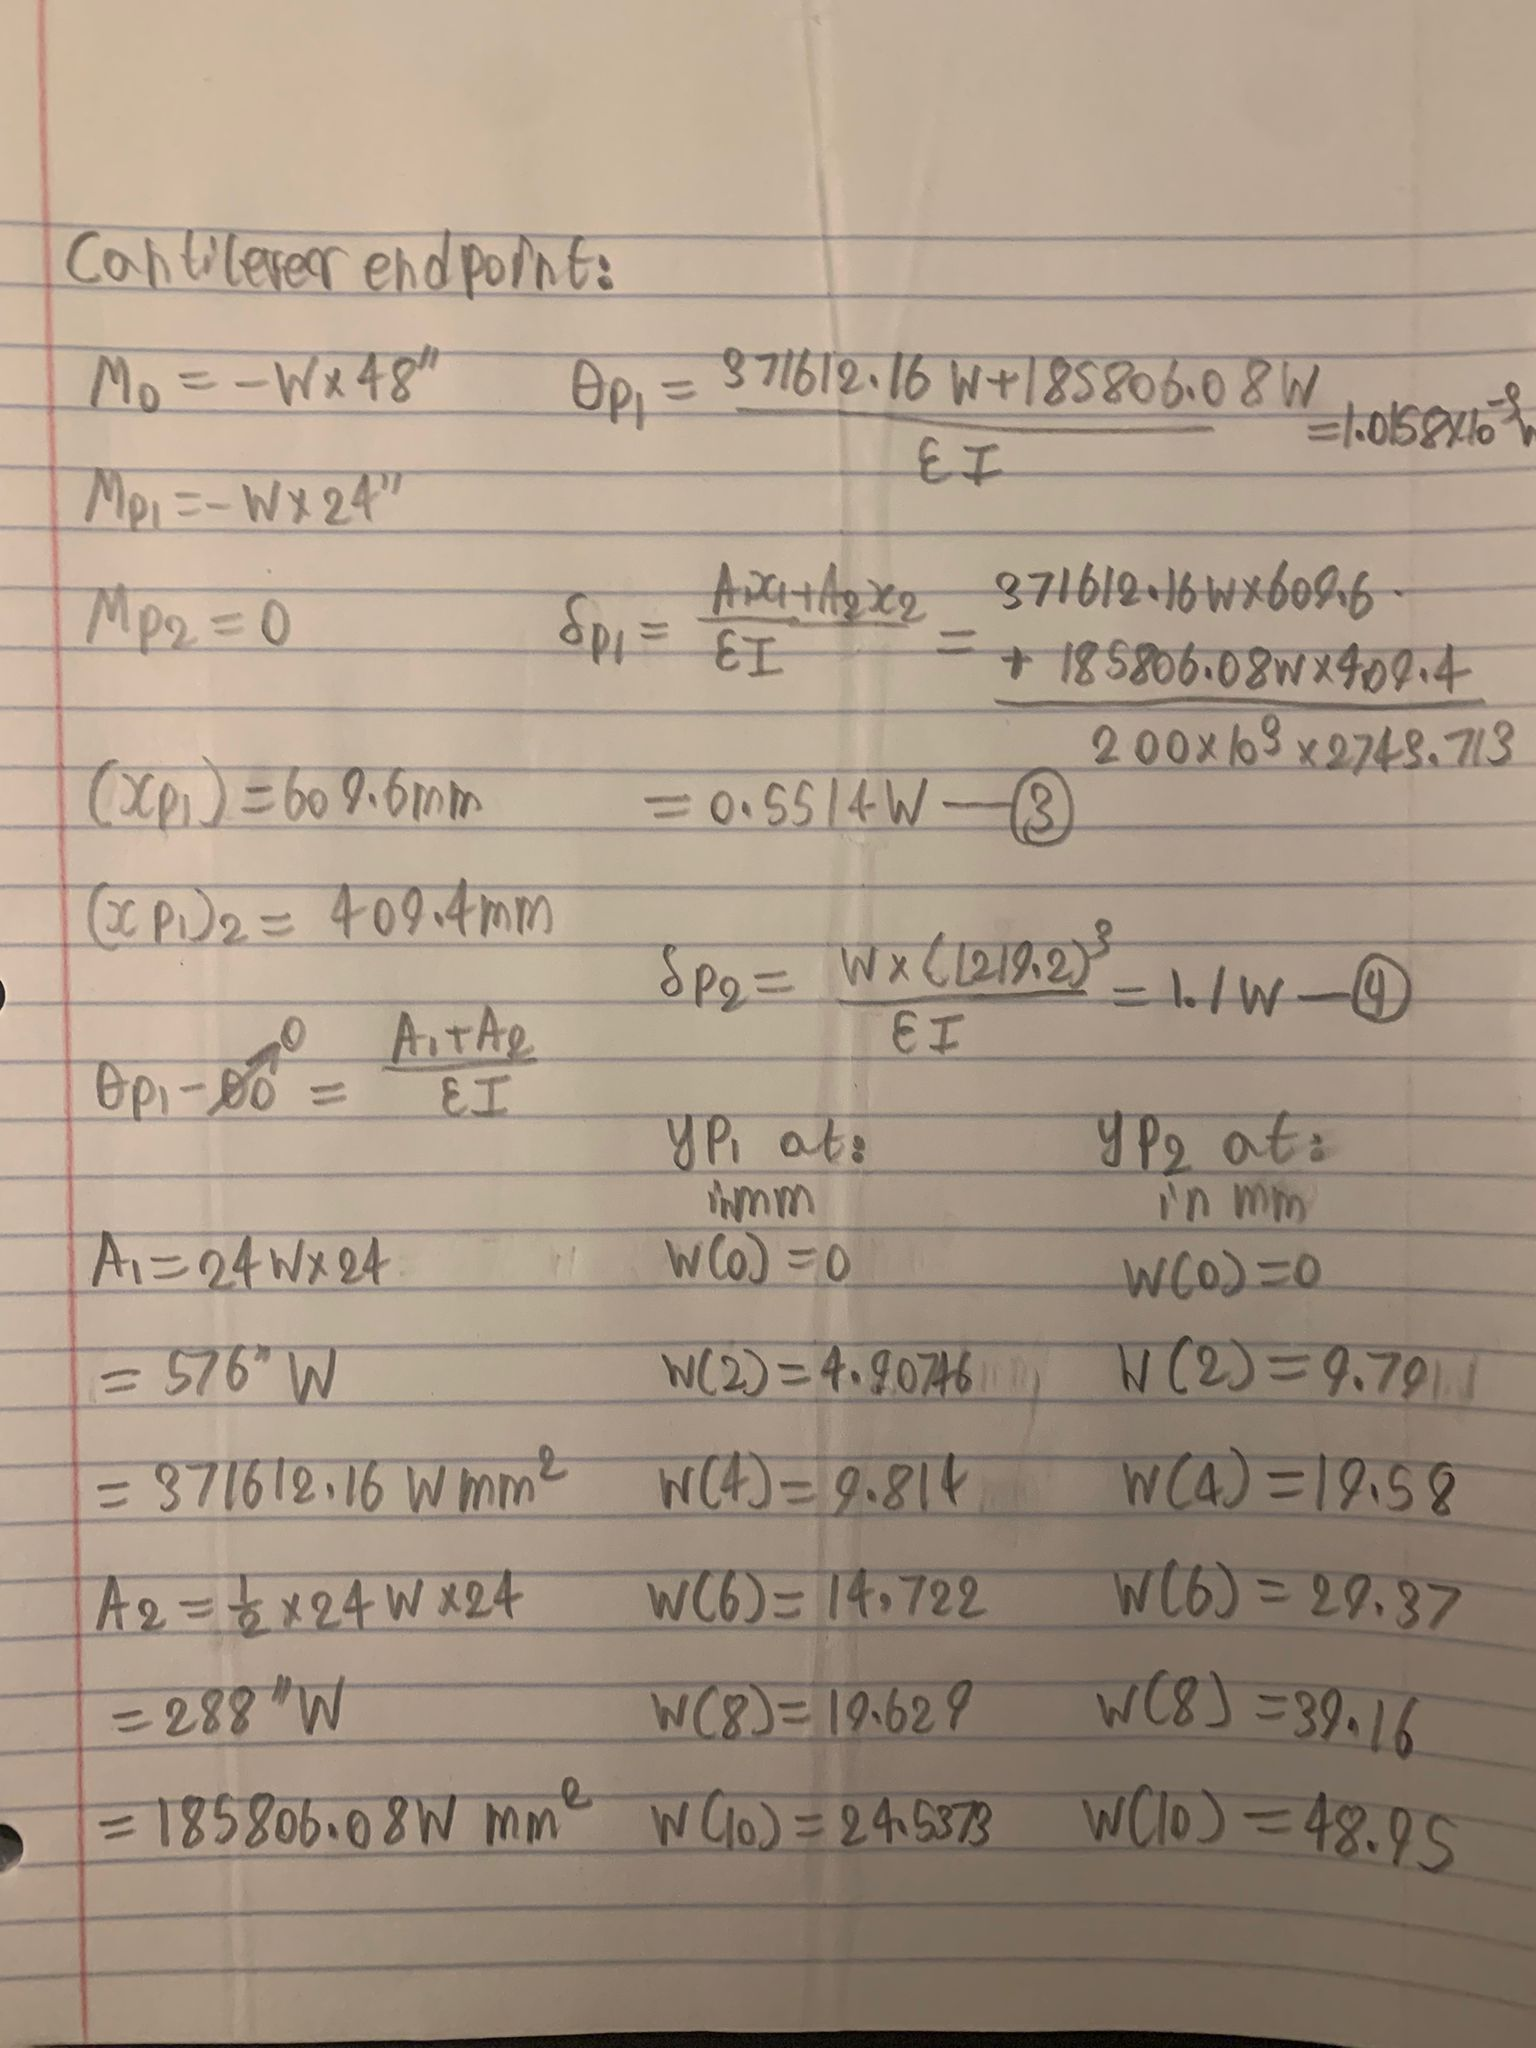
\includegraphics[width=0.6\textwidth]{./Images/C_E.jpeg}
    \caption{Theoretical deflection of the cantilever beam at the end}
    \label{fig:TheoreticalCantileverBeamEnd}
\end{figure}
\newpage
\subsubsection{Experimental Results}
The experimental results for the deflection of the cantilever beam with the
load applied at the end are shown in table \ref{tab:ExperimentalCantileverBeamEnd}.
\begin{table}[H]
    \centering
    \caption{Experimental deflection of the cantilever beam at the end}
    \label{tab:ExperimentalCantileverBeamEnd}
    \begin{tabular}{|c|c|c|}
        \hline
        \textbf{Load (lb)} & \textbf{Deflection P1 (in)} & \textbf{Deflection P2 (in)}\\
        \hline
        2 & -0.038511811 & -0.085669291 \\
        \hline
        4 & -0.078137795 & -0.183468504 \\
        \hline
        6 & -0.120314961 & -0.297409449 \\
        \hline
        8 & -0.161791339 & -0.398330709 \\
        \hline
        10 & -0.205374016 & -0.506389764 \\
        \hline
    \end{tabular}
\end{table}
\subsubsection{Comparison of Theoretical and Experimental Results}
To compare the theoretical and experimental results, the theoretical deflection
values and the experimental deflection values are shown in table \ref{tab:ComparisonCantileverBeamEnd}.
\begin{table}[H]
  \centering
  \caption{Comparison of theoretical and experimental deflection of the cantilever beam at the end}
  \label{tab:ComparisonCantileverBeamEnd}
  \begin{adjustwidth}{-1in}{-1in}
    \begin{tabular}{|c|c|c|c|}
        \hline
        \textbf{Load (lb)} & \textbf{Theoretical Deflection (in)} & \textbf{Experimental Deflection (in)} & \textbf{Percentage Error (\%)} \\
        \hline
        0 & 0 & 0 & 0 \\
        \hline
        2 & -0.38568 & -0.30539 & 20.8195 \\
        \hline
        4 & -0.77137 & -0.61644 & 20.084 \\
        \hline
        6 & -1.15705 & -0.91759 & 20.6953 \\
        \hline
        8 & -1.154273 & -1.23997 & 19.625 \\
        \hline
        10 & -1.923842 & -1.53019 & 20.6507 \\
        \hline
    \end{tabular}
  \end{adjustwidth}
\end{table}
\newpage
The difference is also plotted in figure \ref{fig:ComparisonCantileverBeamEnd}.
\begin{figure}[H]
    \centering
    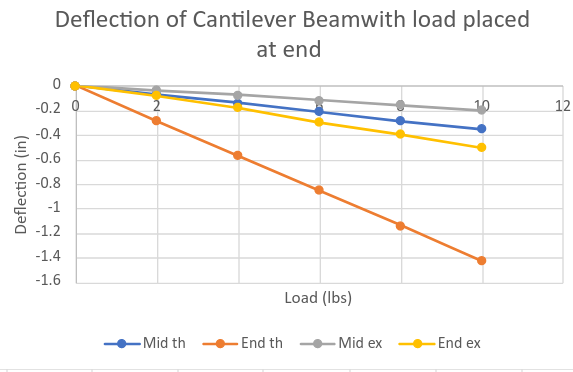
\includegraphics[width=0.9\textwidth]{./Images/C_E_C.png}
    \caption{Comparison of theoretical and experimental deflection of the cantilever beam at the end}
    \label{fig:ComparisonCantileverBeamEnd}
\end{figure}
\newpage
\subsection{Simply Supported Beam Load Applied at the Mid-Span}
\subsubsection{Theoretical Results}
The calculations for the theoretical deflection of the simply supported beam
with the load applied at the mid-span are shown in figure
\ref{fig:TheoreticalSimplySupportedBeamMid}.
\begin{figure}[H]
    \centering
    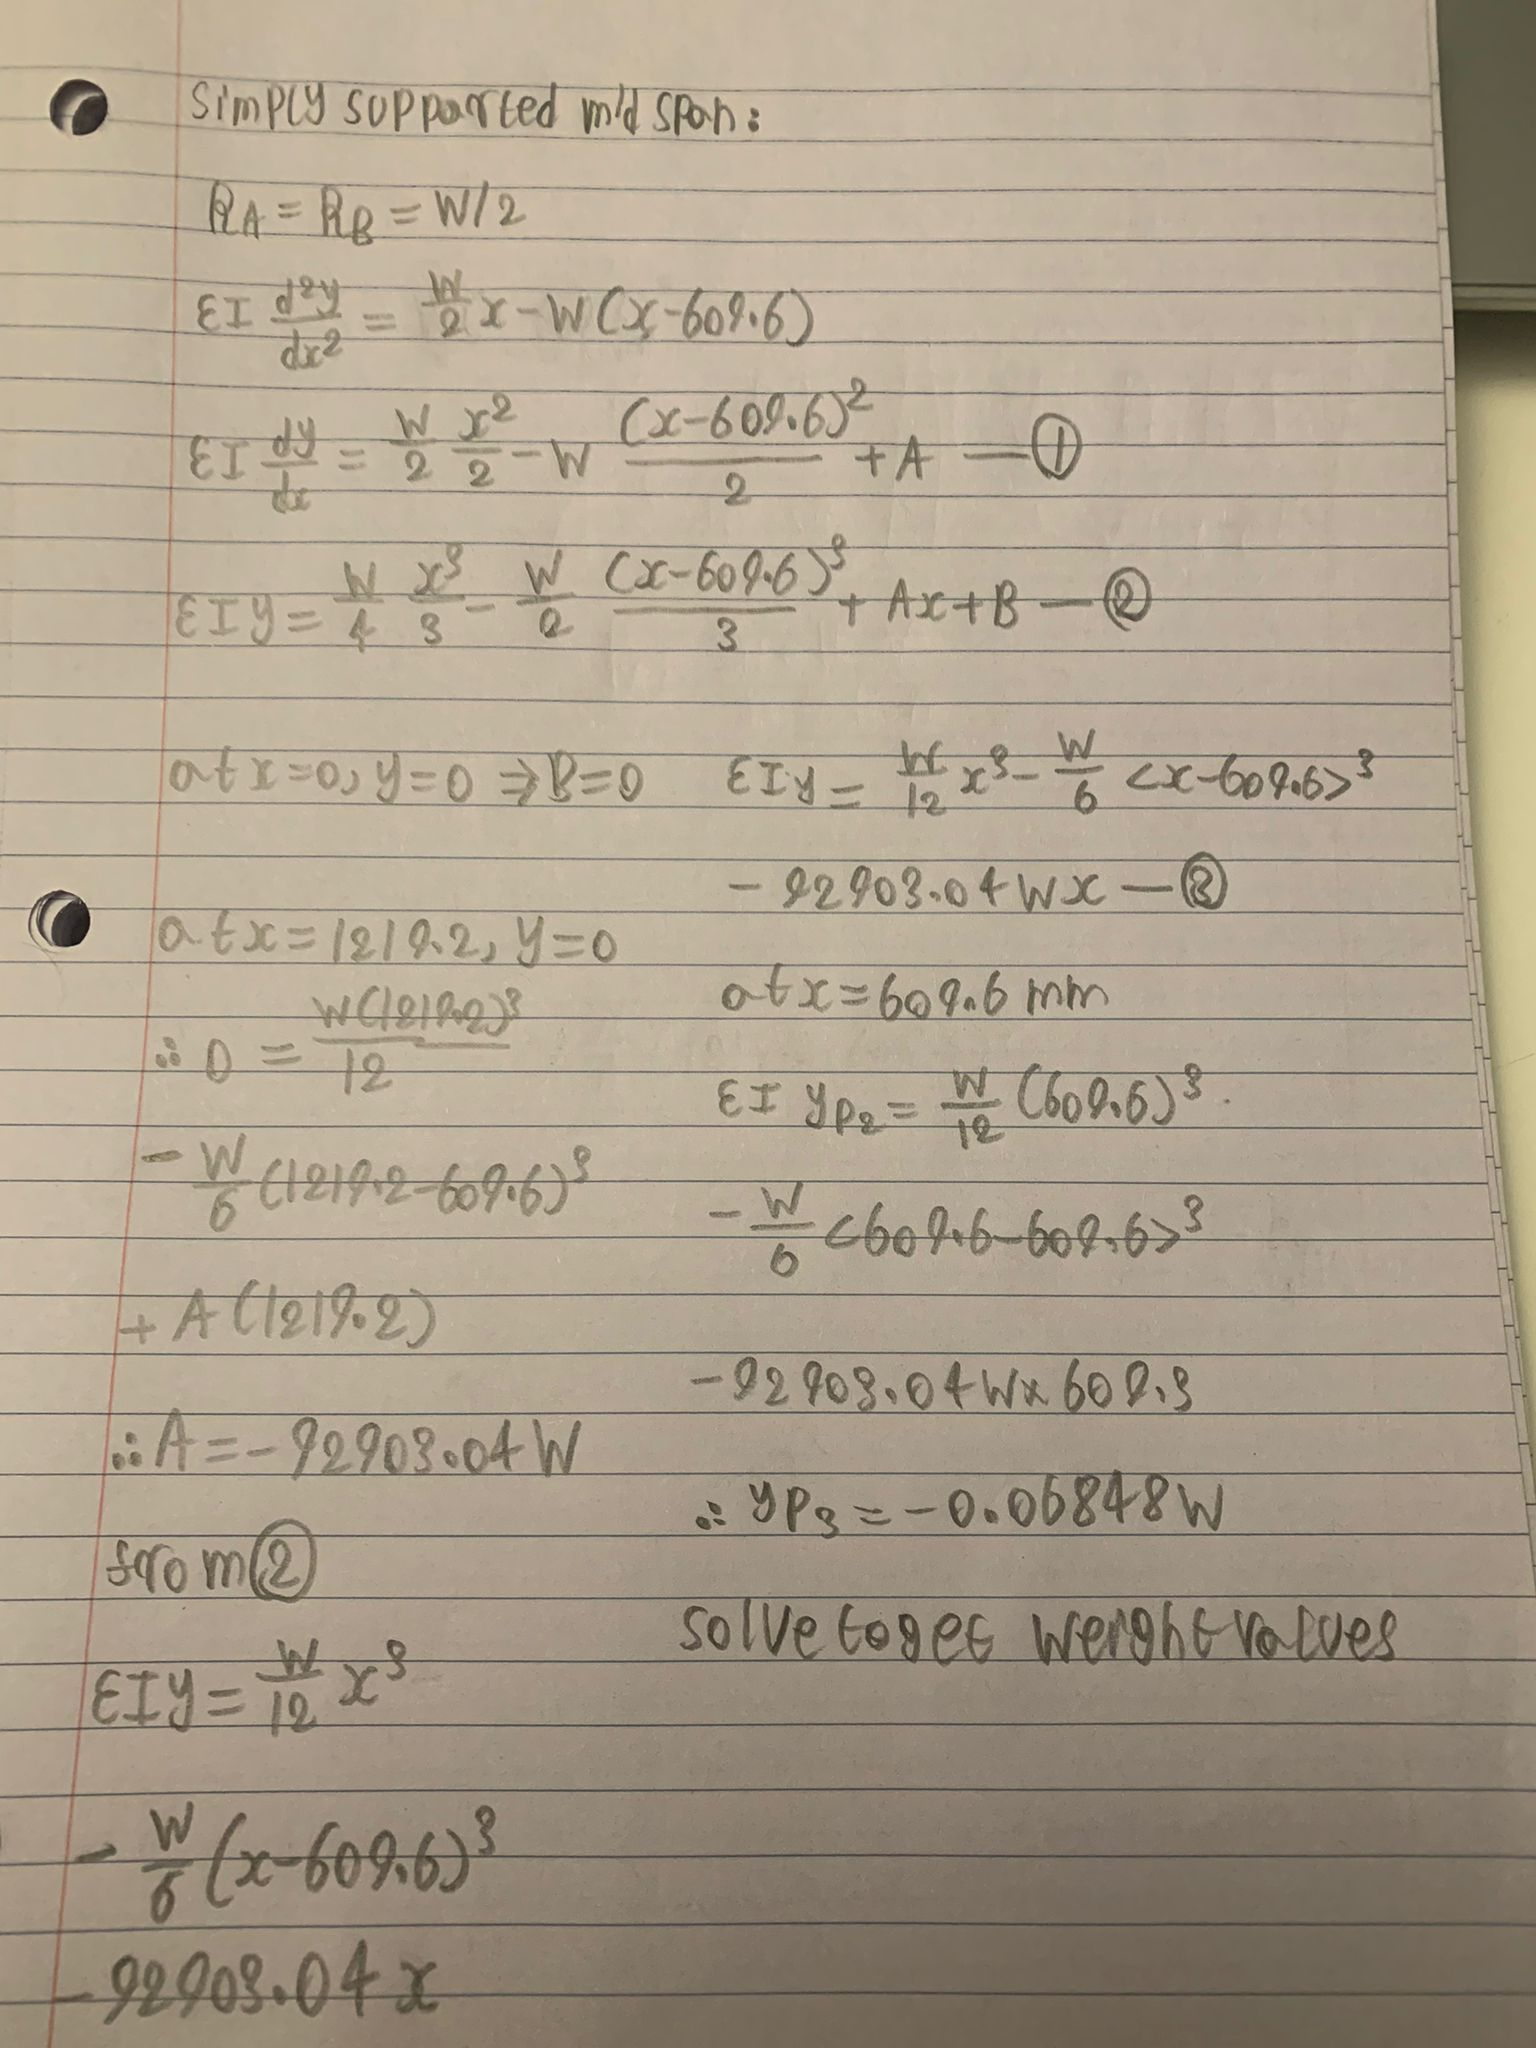
\includegraphics[width=0.6\textwidth]{./Images/S_M.jpeg}
    \caption{Theoretical deflection of the simply supported beam at the mid-span}
    \label{fig:TheoreticalSimplySupportedBeamMid}
\end{figure}
\newpage
\subsubsection{Experimental Results}
The experimental results for the deflection of the simply supported beam with
the load applied at the mid-span are shown in table
\ref{tab:ExperimentalSimplySupportedBeamMid}.
\begin{table}[H]
    \centering
    \caption{Experimental deflection of the simply supported beam at the mid-span}
    \label{tab:ExperimentalSimplySupportedBeamMid}
    \begin{tabular}{|c|c|c|}
        \hline
        \textbf{Load (lb)} & \textbf{Deflection P1 (in)} & \textbf{Deflection P2 (in)}\\
        \hline
        10 & -0.073925197 & -0.068783465 \\
        \hline
        20 & -0.152350394 & -0.13619685 \\
        \hline
        30 & -0.23169685 & -0.202275591 \\
        \hline
        40 & -0.313082677 & -0.268098425 \\
        \hline
    \end{tabular}
\end{table}
\subsubsection{Comparison of Theoretical and Experimental Results}
To compare the theoretical and experimental results, the theoretical deflection
values and the experimental deflection values are shown in table \ref{tab:ComparisonSimplySupportedBeamMid}.
\begin{table}[H]
  \centering
  \caption{Comparison of theoretical and experimental deflection of the simply supported beam at the mid-span}
  \label{tab:ComparisonSimplySupportedBeamMid}
  \begin{adjustwidth}{-1in}{-1in}
    \begin{tabular}{|c|c|c|c|}
        \hline
        \textbf{Load (lb)} & \textbf{Theoretical Deflection (in)} & \textbf{Experimental Deflection (in)} & \textbf{Percentage Error (\%)} \\
        \hline
        0 & 0 & 0 & 0 \\
        \hline
        10 & -0.120525977 & -0.073925197 & 38.66451143 \\
        \hline
        20 & -0.241051954 & -0.152350394 & 36.79769396 \\
        \hline
        30 & -0.361577931 & -0.23169685 & 35.92063273 \\
        \hline
        40 & -0.482103908 & -0.313082677 & 35.05908748 \\
        \hline
    \end{tabular}
  \end{adjustwidth}
\end{table}
\newpage
The difference is also plotted in figure \ref{fig:ComparisonSimplySupportedBeamMid}.
\begin{figure}[H]
    \centering
    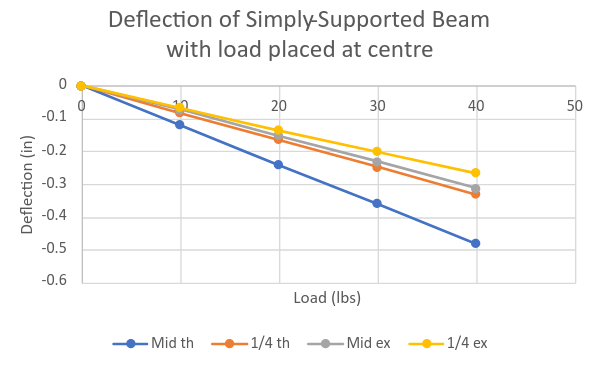
\includegraphics[width=0.9\textwidth]{./Images/S_M_C.png}
    \caption{Comparison of theoretical and experimental deflection of the simply supported beam at the mid-span}
    \label{fig:ComparisonSimplySupportedBeamMid}
\end{figure}
\newpage
\subsection{Simply Supported Beam Load Applied at the Quarter-Span}
\subsubsection{Theoretical Results}
The calculations for the theoretical deflection of the simply supported beam
with the load applied at the quarter-span are shown in figure
\ref{fig:TheoreticalSimplySupportedBeamQuarter}.
\begin{figure}[H]
    \centering
    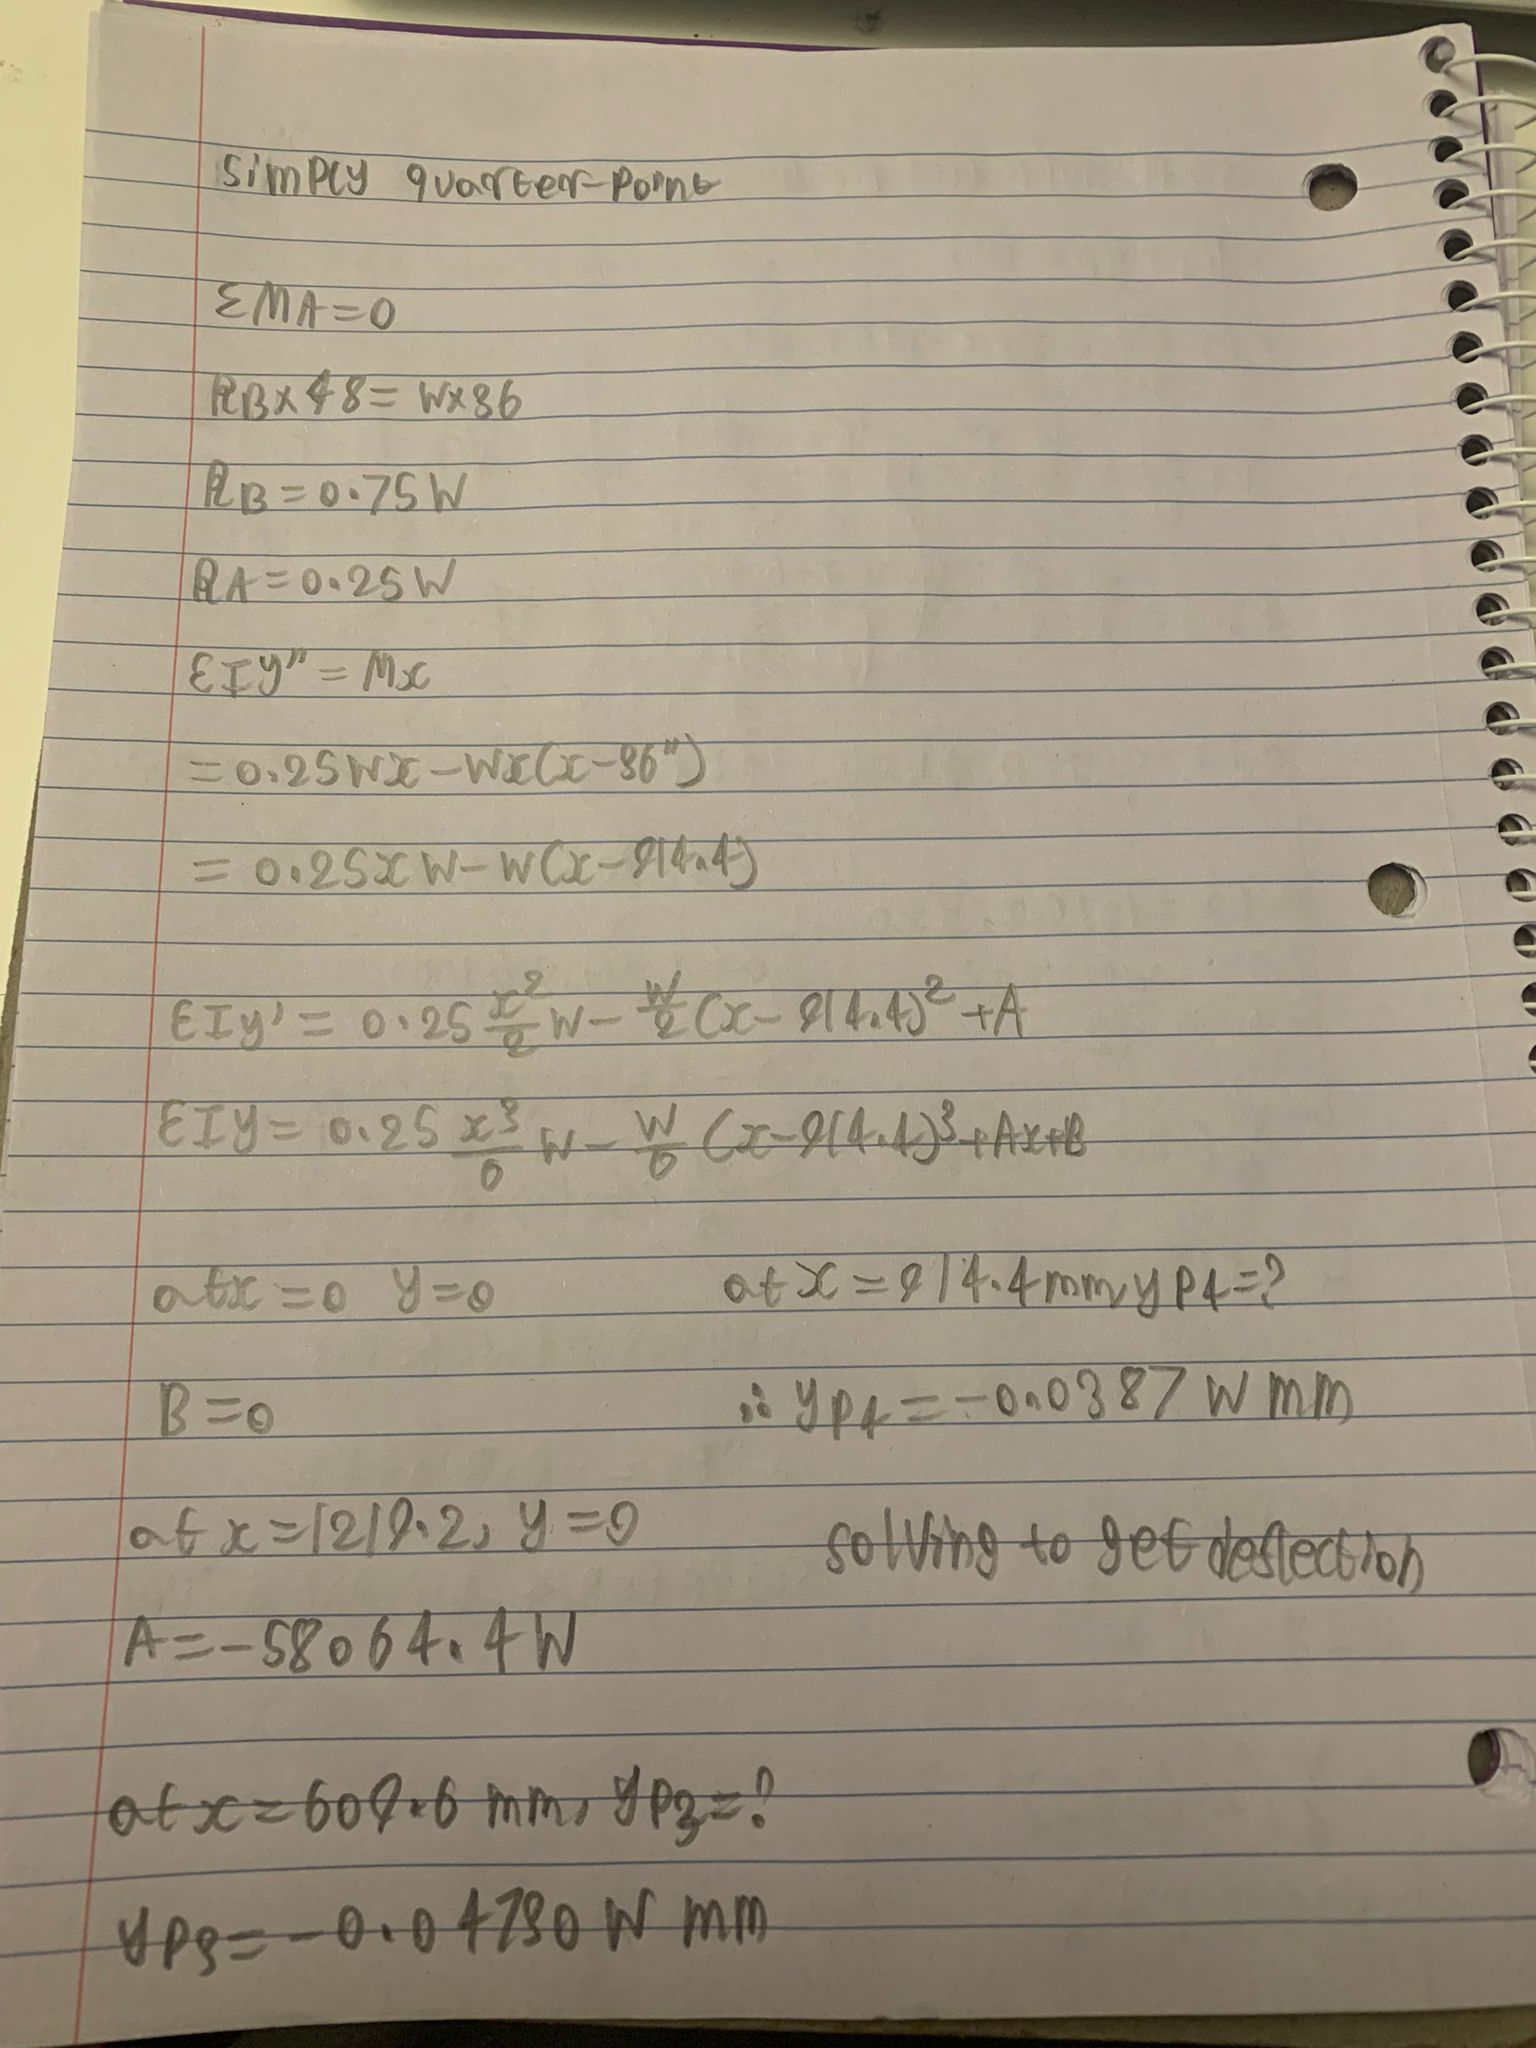
\includegraphics[width=0.6\textwidth]{./Images/S_Q.jpeg}
    \caption{Theoretical deflection of the simply supported beam at the quarter-span}
    \label{fig:TheoreticalSimplySupportedBeamQuarter}
\end{figure}
\newpage
\subsubsection{Experimental Results}
The experimental results for the deflection of the simply supported beam with
the load applied at the quarter-span are shown in table
\ref{tab:ExperimentalSimplySupportedBeamQuarter}.
\begin{table}[H]
    \centering
    \caption{Experimental deflection of the simply supported beam at the quarter-span}
    \label{tab:ExperimentalSimplySupportedBeamQuarter}
    \begin{tabular}{|c|c|c|}
        \hline
        \textbf{Load (lb)} & \textbf{Deflection P1 (in)} & \textbf{Deflection P2 (in)}\\
        \hline
        10 & -0.018897638 & -0.018897638 \\
        \hline
        20 & -0.039370079 & -0.039370079 \\
        \hline
        30 & -0.05984252 & -0.05984252 \\
        \hline
        40 & -0.080314961 & -0.080314961 \\
        \hline
    \end{tabular}
\end{table}
\subsubsection{Comparison of Theoretical and Experimental Results}
To compare the theoretical and experimental results, the theoretical deflection
values and the experimental deflection values are shown in table \ref{tab:ComparisonSimplySupportedBeamQuarter}.
\begin{table}[H]
  \centering
  \caption{Comparison of theoretical and experimental deflection of the simply supported beam at the quarter-span}
  \label{tab:ComparisonSimplySupportedBeamQuarter}
  \begin{adjustwidth}{-1in}{-1in}
    \begin{tabular}{|c|c|c|c|}
        \hline
        \textbf{Load (lb)} & \textbf{Theoretical Deflection (in)} & \textbf{Experimental Deflection (in)} & \textbf{Percentage Error (\%)} \\
        \hline
        0 & 0 & 0 & 0 \\
        \hline
        10 & -0.120525977 & -0.018897638 & 24.3305 \\
        \hline
        20 & -0.241051954 & -0.039370079 & 23.628 \\
        \hline
        30 & -0.361577931 & -0.05984252 & 23.452 \\
        \hline
        40 & -0.482103908 & -0.080314961 & 23.332 \\
        \hline
    \end{tabular}
  \end{adjustwidth}
\end{table}
\newpage
The difference is also plotted in figure \ref{fig:ComparisonSimplySupportedBeamQuarter}.
\begin{figure}[H]
    \centering
    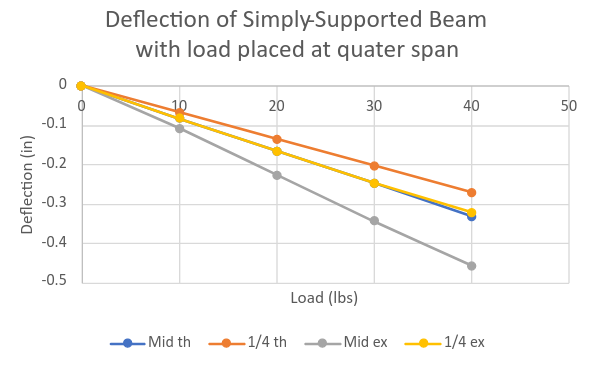
\includegraphics[width=0.9\textwidth]{./Images/S_Q_C.png}
    \caption{Comparison of theoretical and experimental deflection of the simply supported beam at the quarter-span}
    \label{fig:ComparisonSimplySupportedBeamQuarter}
\end{figure}
\newpage
\section{Discussion}
\subsection{Analysis of Results}
The comparison of the theoretical and experimental results showed that the
percentage error is around 20\% for most the cases. This is a significant
difference, the reason can be found in the sources of error section.
\subsection{Sources of Error}
The sources of error for this experiment are listed as follows:
\begin{enumerate}
    \item \textbf{Material Properties:} The theoretical calculations assume
      that the beam is made of a homogeneous material with uniform properties.
      However, the actual beam is made of a composite material with varying
      properties. This difference in material properties can cause the
      theoretical calculations to be inaccurate.
    
    \item \textbf{Beam Geometry:} The theoretical calculations assume that the
      beam is a perfect rectangle with uniform cross-section. However, the
      actual beam is not a perfect rectangle and has varying cross-section
      along its length. This difference in beam geometry can cause the
      theoretical calculations to be inaccurate.
    
    \item \textbf{Experimental Errors:} The experimental measurements are
      subject to errors due to the limitations of the measuring instruments.
      This can cause the experimental results to be inaccurate.
\end{enumerate}
\newpage
\section{Conclusions}
\subsection{Summary}
The deflection of beams under different loading conditions is a fundamental
aspect of structural engineering. In this experiment, the deflection of two
different beam configurations, the cantilever and the simply supported beam,
were investigated both theoretically and experimentally. The deflection of
these beams were measured under varying loads and the theoretical and
experimental results were compared to assess the accuracy and reliability of
the theoretical models in predicting structural deflections.\\[10pt]
The objectives for this experiment were outlined as follows:
\begin{enumerate}
    \item \textbf{Measurement of Deflection:} Experimentally acquire accurate
      values of deflection for both a cantilever and a simply supported beam
      under varying loads to understand their structural behaviors.
    
    \item \textbf{Comparison of Experimental and Theoretical Results:} Analyze
      and compare the obtained experimental deflection values with the
      theoretically predicted values for both the cantilever and the simply
      supported beam to assess the accuracy and reliability of theoretical
      models in predicting structural deflections.
\end{enumerate}
The results of this experiment showed that the theoretical and experimental
deflection values are not in agreement. The percentage error between the
theoretical and experimental results was around 20\% for most of the cases.
This difference in the results can be attributed to the following sources of
error: the difference in material properties, the difference in beam geometry,
and the experimental errors.
\subsection{Maxwell's Law of Reciprocal Deflections}
Maxwell's law of reciprocal deflections states that the deflection at any point
in a beam is equal to the deflection at the same point in a beam with the
loading and supports interchanged. This law was verified in this experiment by
comparing the deflection of the cantilever beam with the load applied at the
mid-span and the deflection of the cantilever beam with the load applied at the
end. The deflection values at the mid-span (\(P1\)) and at the end of the
cantilever beam (\(P2\)) were measured for both loading conditions. The
theoretical deflection values were also calculated for both loading conditions.
The comparison of the theoretical and experimental results showed that the
deflection values at the mid-span (\(P1\)) and at the end of the cantilever
beam (\(P2\)) are equal for both loading conditions. This verifies Maxwell's
law of reciprocal deflections.
\end{document}
